\chapter{Introduction}

Our understanding of the phenomenon of diffraction really begins with Huygens' famous construction, now known as Huygens' principle. This states that each point on a propagating wavefront can be considered as a secondary source radiating a spherical wave. The transverse polarization of the radiated wave was not apparent to Huygens; nor was the principle of wave interference, which had to wait more than a hundred years for Thomas Young to discover it. Augustin Fresnel then combined the ideas of Huygens and Young in order to describe the nature of the light diffracted by various aperture, such as a knife edge, an opaque strip, and a parallel-sided opening. This last example provides a useful introduction to the phenomenon of diffraction and its application to aperture antenna.

\section{An Elementary Example of Diffraction}
\label{sec:eg}
Consider a plane electromagnetic wave incident normally on a parallel-sided slit cut in a thin perfectly conducting plane, as in Fig.\ \ref{fig:huymtd}.
\begin{figure}[htbp]
	\begin{center}
		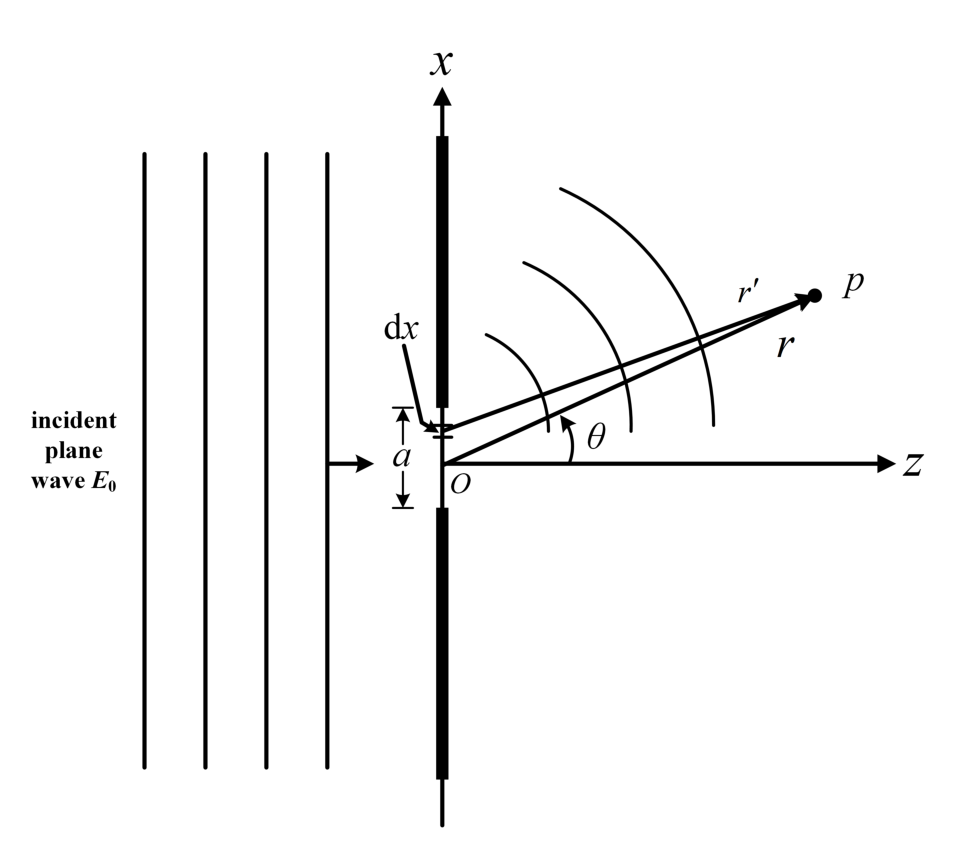
\epsfig{width=3.5in,file=Figs/intro/huy.eps}
	\end{center}
	\caption{Plane wave diffracted by a parallel-sided slit cut in a perfectly conducting plane. Huygens representation.}
	\label{fig:huymtd}
\end{figure}
For this two-dimensional situation a typical element of width $\mathrm{d}x$ in the aperture formed by the slit can be supposed, by an obvious modification of Huygens' principle, to radiate a cylindrical wave into the medium to the right of the aperture plane. It is reasonable to assume that the strength of the secondary source is proportional to the magnitude $E_0$ of the field incident on the aperture from the left, and to the elemental width $\mathrm{d}x$. Then, without bothering with any refinement at this stage, the contribution of the element $E_0\mathrm{d}x$ to the field at a point $p$ a distance $r'$ away is
\begin{equation}
\mathrm{d}E_p = CE_0\mathrm{d}x \frac{1}{\sqrt{r'}} \exp(-jkr'), 
\label{eq:huyprp}
\end{equation}
where $C$ is a constant and $k$ is the phase retardation per unit distance suffered by a wave traveling in the medium to the right of the aperture plane at the frequency of the incident field. If the distance $r$ of the point $p$ from the center $O$ of the aperture is very large, in comparison with the aperture width $a$, it is legitimate to replace $r'$ by $r$ under the square root, and $r'$ by $r-xsin\theta$ in the phase term of equation (\ref{eq:huyprp}). (The direction $Op$ makes and angle $\theta$ to the axis normal to the aperture). Then, integrating over the width of the aperture, the total diffracted field at $p$ is
\begin{equation}
E_p = \frac{CE_0}{\sqrt{r}}\exp(-jkr)\int_{-a/2}^{a/2}\exp(jkx\sin\theta)\mathrm{d}x
\label{eq:ffsub}
\end{equation}
so that
\begin{equation}
E_p = \frac{CE_0a}{\sqrt{r}}\exp(-jkr)
	\frac{\sin({\dfrac{\pi a\sin\theta}{\lambda}})}
		 {(\dfrac{\pi a\sin\theta}{\lambda})}
\label{eq:ffexpr}
\end{equation}
Thus Huygens' principle embodied in equation (\ref{eq:huyprp}) gives the field at $p$ as a superposition of cylindrical waves from all parts of the aperture (equation (\ref{eq:ffsub})) which produces the interference pattern of equation (\ref{eq:ffexpr}).

This equation reveals that the field at the distance point $p$ diffracted by the aperture at $O$ is basically a cylindrical waves centered on $O$, with an angular dependency of the form $(\sin \psi)/\psi$ where $\psi = \pi a\sin \theta/\lambda$. The angular dependence has a characteristic lobe structure, with the main lobe having its maximum in the direction $\theta=0$, and with zeros at angles given by $\sin \theta = \pm \lambda/a, \pm2\lambda/a$, and so on.

The uniformly illuminated slit is a useful elementary model of an aperture antenna, which is a class of antennas that is widely used at microwave frequencies for communication and radar surveillance. Thus it is immediately apparent from equation (\ref{eq:ffexpr}) that the level of the radiated field depends on the aperture width, increasing as {\itshape a} increases. At the same time the angular width of the main lobe is correspondingly reduced. In antenna parlance (see section \ref{sec:antconc}), as the aperture width is increased, the gain of the antenna is increased and its beamwidth is reduced.

\section{Diffraction Theory By Plane Wave}
Developments in diffraction theory have been dominated by the ideas of Huygens and Fresnel. So, although considerable refinements have been achieved (see Stratton (1941), for example) in Kirchioff's scalar theory of diffraction and then in Stratton and Chu's vector theory, the underlying principle of spherical waves radiated by known fields has remained. This is understandable in view of the simplicity and strength of Huygen's original idea. But it has meant that the student of diffraction has been presented with some difficult mathematical hurdles to clear before he can obtain some familiarity with the phenomenon of diffraction.

The difficult seems to arise from the fact that whereas spherical waves are a natural physical entity, they are rather clumsy from a mathematical point of view. In contrast, the plane wave, which is a simple mathematical entity, can never exist as such in the real physical world. However, it has long been known that naturally occurring fields can be {\itshape represented} by the superposition of either a discrete set or a continuum of plane waves traveling in different directions. Perhaps the simplest and best know example of this is the field in a rectangular waveguide, which is given precisely by the superposition of two plane waves traveling in directions equally incident to the waveguide axis (see Appendix \ref{sec:wg}). In general such a set of plane waves is know as an angular spectrum.

In this book we shall be using the angular plane-wave spectrum concept to develop the theory of diffraction. This approach is not only relatively simple mathematical, as already indicated, but it is also fundamentally more precise than older theories of diffraction. This is because the approximations that must inevitably be made occur at a large stage of the analysis in the case of the plane-wave approach.

One conceptual difficulty concerning the physical plausibility of the angular spectrum method must be dealt with right away. It is that, since plane waves are of infinite lateral extent, it may seem strange at first sight that they can be used to represent realistic fields. But the situation is no different, in principle, from the representation of an arbitrary time waveform $f(t)$ by the superposition of a set of ideal sinusoids. In that case, if the amplitude spectrum as a function of frequency ${\omega}$ is $F({\omega})$ then the waveform is given by the Fourier integral, 
\begin{equation}
f(t)=\frac{1}{2\pi}\int_{-\infty}^{\infty}F(\omega)\exp(j\omega t)d\omega.
\label{eq:ft}
\end{equation}
The individual sinusoids in the integrand of this equation are of infinite duration in time, whereas the waveform $f(t)$ that they represent is usually of finite duration. An immediate advantage of the Fourier integral of equation (\ref{eq:ft}) is that it can be inverted to give
\begin{equation}
F(\omega)=\int_{-\infty}^{\infty}f(t)\exp(-j\omega t)dt.
\end{equation}
A similar advantage occurs in using the angular plane-wave spectrum to represent radiated fields, as the following outline analysis shows.

Suppose, instead of the cylindrical waves of Fig. \ref{fig:huymtd}, the field diffracted by a slit is represented as the superposition of a set of plane waves, of which a typical member is that shown in Fig. \ref{fig:angspe}. The angle $\theta$ is now a variable describing the directions of the component plane waves constituting the angular spectrum.
\begin{figure}[htbp]
	\begin{center}
		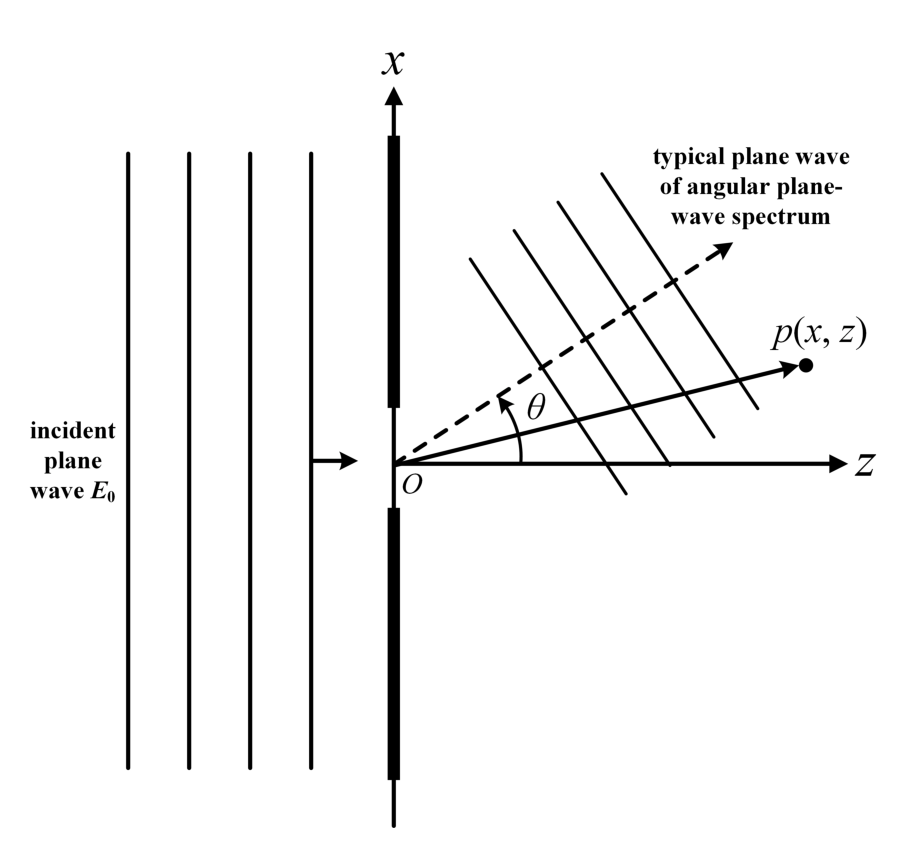
\epsfig{width=3.5in,file=Figs/intro/angspe.eps}
	\end{center}
	\caption{A plane wave diffracted by a slit. Plane-wave spectrum representation.}
	\label{fig:angspe}
\end{figure}
For technical reasons direction will be specified by $\sin \theta$ rather than $\theta$. Then if the set of plane waves is described by the spectrum function $F(\sin \theta)$, the contribution of this single plane wave of elementary amplitude $F(\sin \theta)\mathrm{d}(\sin \theta)$ to the field at some point $p$ is
\begin{equation}
\mathrm{d}E_p(x,z)=F(\sin \theta)\mathrm{d}(\sin \theta)\exp\{-jk(x\sin \theta+z\cos \theta)\}
\end{equation}
The complete field at $p$ is then obtained by integration as 
\begin{equation}
E_p(x,z)=\int_{-\infty}^{\infty}F(\sin \theta)\exp\{-jk(x\sin \theta+z\cos \theta)\}\mathrm{d}(\sin \theta)
\label{eq:compl}
\end{equation}
(For present purposes it may be assumed that the range of integration is artificially extended beyond its natural limits of $\pm1$ for analytical convenience. However, it will be shown in Chapter \ref{ch:pw2d} that waves traveling in directions such that $|\sin \theta| > 1$ are far from artificial). Now, defining the field over the aperture as
\begin{equation}
f(x)=E_p(x,0),
\label{eq:ataper}
\end{equation} 
equations \ref{eq:compl} and \ref{eq:ataper} can be combined to give
\begin{equation}
f(x)=\int_{-\infty}^{\infty}F(\sin\theta)\exp(-jkx\sin\theta)\mathrm{d}(\sin\theta)
\end{equation}
This is a Fourier integral that can be inverted to give the angular spectrum $F(\sin\theta)$ in terms of the aperture field $f(x)$ as
\begin{equation}
F(\sin\theta)=\frac{1}{\lambda}\int_{-\infty}^{\infty}f(x)\exp(jkx\sin\theta)\mathrm{d}x
\label{eq:spefun}
\end{equation}

In the elementary diffraction example of section \ref{sec:eg} the aperture field is assumed to be non-zero only across the slit, so that
\begin{equation}
f(x)= \left\{
\begin{array}{ll}
E_0 & \text{for }|x| \leqslant a/2 \\
0 & otherwise
\end{array}
\right.
\end{equation}
Substituting this into equation (\ref{eq:spefun}) yields the angular spectrum
\begin{equation}
\begin{aligned}
F(\sin\theta)&=\frac{E_0}{\lambda}\int_{-a/2}^{a/2}\exp(jkx\sin\theta)\mathrm{d}x\\
&=\frac{E_0a}{\lambda}\frac{\sin(\dfrac{\pi a\sin\theta}{\lambda})}{(\dfrac{\pi a\sin\theta}{\lambda})}
\end{aligned}
\end{equation}
which has the same angular dependence as the far field of equation (\ref{eq:ffexpr}) derived from Huygen's principle. Thus we can seen in this particular example, and will later establish as generally true, that the angular spectrum gives the far field of the radiation. And furthermore, as equation (\ref{eq:spefun}) shows, the angular spectrum is simply the Fourier transform of the field across the radiation aperture. Once $F(\sin\theta)$ is known the radiated field $E_p(x,z)$ at any point to the right of the aperture plane is determined by the integral of equation (\ref{eq:compl}).

The angular plane-wave spectrum representation was popular around the turn of the last century. Rayleigh (1896) used it to describe the fields reflected and transmitted at a corrugated dielectric boundary illuminated by a plane wave, and Debye (1909) used the representation to investigated the fields in the region of a focus. In 1902 Whittaker had proved that the field described by an angular spectrum of plane waves radiating in all directions was a solution of the wave equation. But this form of the angular spectrum leaves the source of radiation unspecified, and is therefore not unique. This limitation was overcome in Weyl's (1919) representation of the field radiating into a half-space bounded by a plane. The source field can be specified over this plane, and so the representation can be unique.

The application of the angular plane-wave spectrum to aperture antenna analysis and synthesis was pioneered by Booker and Clemmow (1950) and Woodward and Lawson (1948), essentially using the Weyl representation in two dimensions. Brown (1958) extended the representation the three dimensions, and introduced a reciprocity theorem for antennas which enabled the concept to be applied to receiving as well as transmitting antennas. This led to a transmitter/receiver coupling formula which applied to near-field coupling as well as to the far field. The angular plane-wave spectrum concept is now used extensively in planar-antenna synthesis (Rhodes, 1974) and in near-field antenna measurements (Paris and Joy, 1978).

In Chapter \ref{ch:pw2d} and \ref{ch:3dfield} of this book the concept of an angular spectrum of plane waves is established for two- and three-dimensional fields. In Chapter \ref{ch:trre} the concept is applied to transmitting antennas, receiving antennas, and the coupling between them. Fresnel diffraction is examined in Chapter \ref{ch:fesnel}, and reflection from flat and curved conducting surfaces in Chapter \ref{ch:refcond}. Particular examples of planar aperture antennas are examined in detail in Chapter \ref{ch:apeant}. Chapter \ref{ch:nonpla} looks briefly at the problem of radiation from non-planar apertures. Appendices provide a summary of the properties of plane waves and of some theorems derived from Maxwell's equations. The remainder of this introductory chapter will be devoted to a physical description of the planar-aperture antennas to be examined in Chapter \ref{ch:apeant}, and to giving a list of those performance characteristics and terms that are in common use in antenna practice.

\section{Some Aperture Antennas}
The following example of microwave antennas used in communications or radar can be described as planar-aperture antennas.\\
\\
\textbf{The Electromagnetic Horn Antenna}\\
At microwave frequencies a simple way of making a radiating antenna is to use an open-ended waveguide with a flared transition section (that is, a horn) added to achieve a reasonable match and increased directivity. (See Fig. \ref{fig:horn}).
\begin{figure}[htbp]
	\begin{center}
		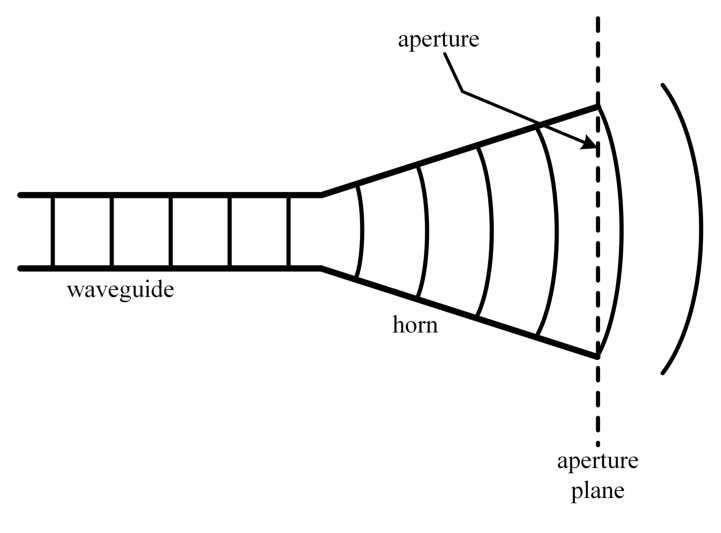
\epsfig{width=3.0in,file=Figs/intro/horn.eps}
	\end{center}
	\caption{The Electromagnetic Horn Antenna. Feint lines indicate equiphase wavefronts of the radiating field.}
	\label{fig:horn}
\end{figure}

An obvious starting point for the analysis of such a radiating device is to assume that the field over the mouth of the horn is an expanded form of the front. Thus the aperture of this antenna is the real aperture formed by the mouth of the horn, assumed to be part of the aperture plane. The field distribution over this plane, the aperture field distribution, could be taken approximately to be the expanded waveguide field over the actual aperture and zero over the remaining part of the aperture plane.

The electromagnetic horn is robust and fairly easy to manufacture. It is widely used as a standard in antenna gain measurements. (For a definition of antenna gain see section \ref{sec:antconc}). But owing to the curvature of the emerging wavefront its gain is relatively low. The different methods that have been devised to correct the curved wavefront of simple primary sources, such as the electromagnetic horn, into the more desirable planar wavefront have led to a variety of antenna designs, of which the horn-lens combination is perhaps the most obvious.\\
\\
\textbf{The Horn-Lens Antenna}\\
\begin{figure}[htbp]
	\begin{center}
		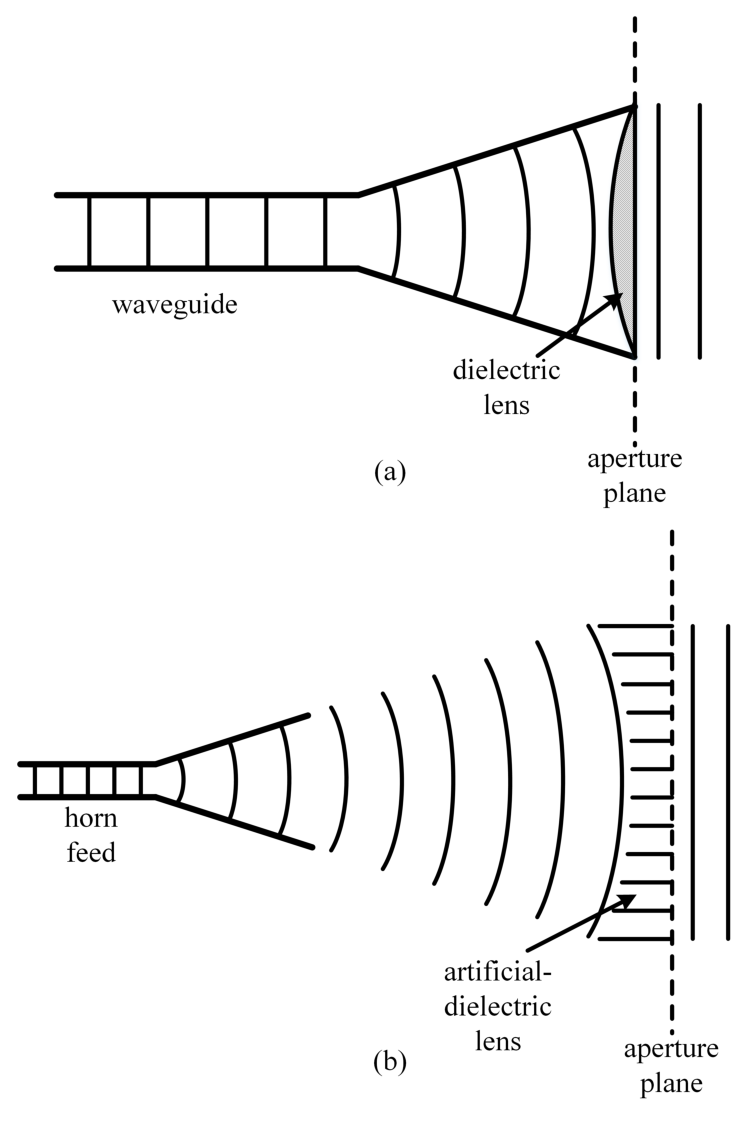
\epsfig{height=4.0in,file=Figs/intro/horn-lens.eps}
	\end{center}
	\caption{The Horn-Lens Antenna. The curved wavefront corrected width (a) a solid dielectric lens, and (b) an artificial-dielectric lens.}
	\label{fig:horn-lens}
\end{figure}
Here the curved wavefront of the field emerging from the mouth of the electromagnetic horn is corrected by the use of a converging lens. The resulting planar wavefront leads to an improvement in the directivity of the radiated field. Two examples are shown in Fig. \ref{fig:horn-lens}).
The solid dielectric lens of Fig. \ref{fig:horn-lens}(a) behaves in exactly the same way as a convex glass lens in optics. The artificial dielectric lens shown schematically in Fig. \ref{fig:horn-lens}(b) consists of a stack of meta-walled waveguides within which the phase velocity of the waves is greater than in air hence the concave construction of the lens. In both cases the natural aperture is just beyond the output face of the lens.

The advantage of the increased directivity and gain are somewhat offset in the horn lens antenna by the reflections that inevitably occur at the front and back surfaces of the lens. The essential robustness of the electromagnetic horn is also diminished in the horn-less combination.\\
\\
\textbf{The Horn-Paraboloid Antenna}\\
An ingenious design which achieves the desired wavefront correction of the field emerging from a horn, without introducing partial reflections and without loss of robustness, is the horn-paraboloid assembly shown in Fig. \ref{fig:horn-para}.
\begin{figure}[htbp]
	\begin{center}
		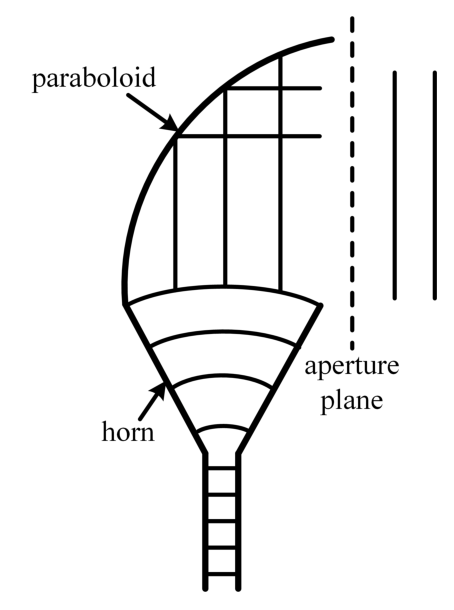
\epsfig{height=3.0in,file=Figs/intro/horn-para.eps}
	\end{center}
	\caption{The Horn-Paraboloid Antenna.}
	\label{fig:horn-para}
\end{figure}
The metal cowl is welded on to the horn and has paraboloidal (this is, part of a parabola of resolution) profile which transforms the spherical wavefront at the mouth of the horn into a planar wavefront which emerges from the side of the assembly. It is convenient in this case to suppose that the radiating aperture of this device lies just beyond the metal structures, as shown in the figure.

However, there is another factor which affects antenna directivity. For maximum directivity the wavefront in the aperture should not only be planar, but as wide as possible. In the antenna designs so far mentioned emphasis has been on correcting the wavefront. We now turn to a series of antenna designs which both correct the wavefront and extend the lateral dimensions of the aperture.\\
\\
\textbf{The Paraboloid Reflector Antenna}\\
This antenna consists of a primary feed, which is shown in Fig \ref{fig:para-ref}. as an electromagnetic horn, positioned at the focus of a paraboloid reflector.
\begin{figure}[htbp]
	\begin{center}
		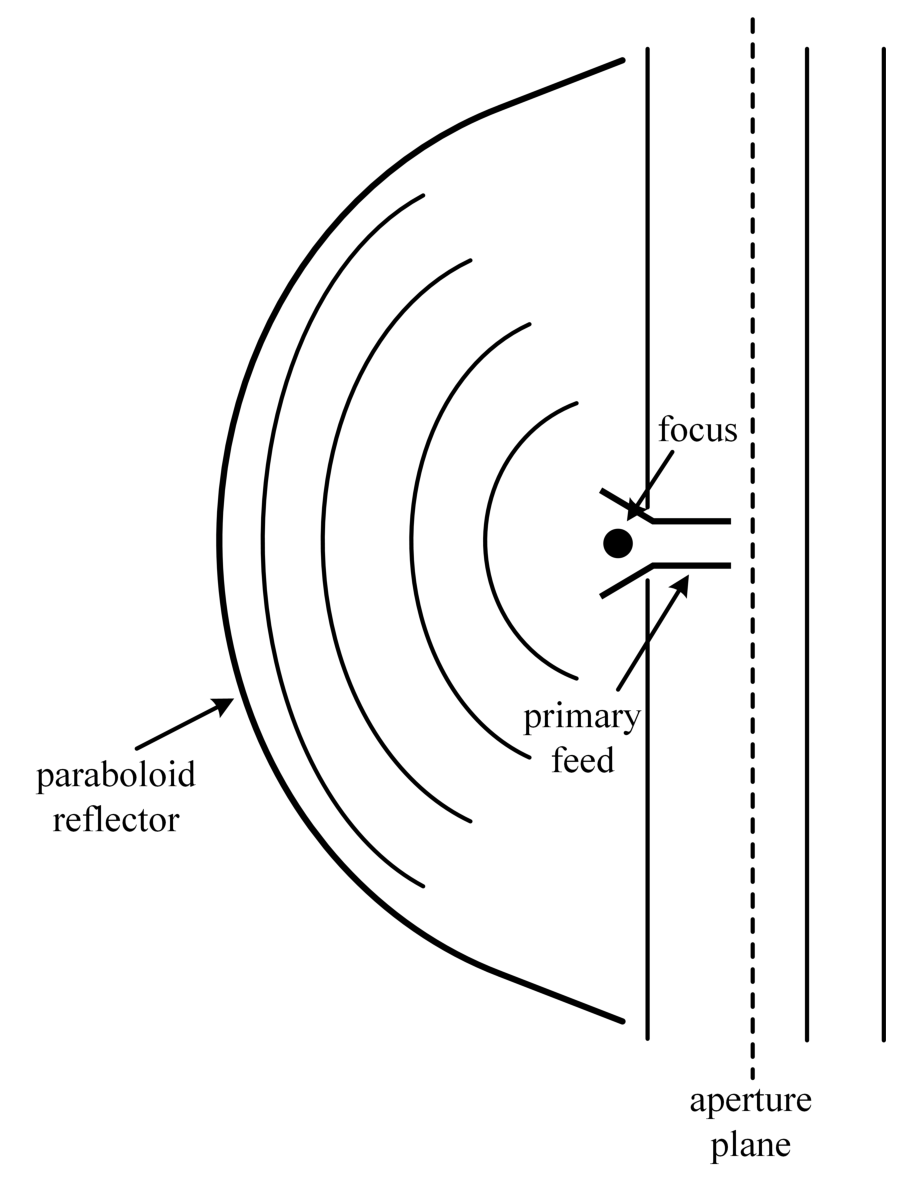
\epsfig{height=3.5in,file=Figs/intro/para-ref.eps}
	\end{center}
	\caption{The Paraboloid Reflector Antenna.}
	\label{fig:para-ref}
\end{figure}
The geometrical properties of the parabola ensure that the spherical wave incident from the feed is transformed into a plane wave on reflection. The lateral extent of the emerging aperture fields, which it is convenient to place beyond the primary feed and its support structure, can be as wide as the lateral extent of the paraboloid.

The simplicity of design (basically that of the searchlight and Newton telescope) and its robustness of construction make the focus-fed paraboloid reflector a very popular choice as a high-gain antenna in communications and radar. However, the physical presence between the reflector and the supposed aperture of the primary feed, its feeder waveguide and its associated support structure, give rise to some deterioration in performance, and to some rather unsatisfactory modifications to the analysis, in comparison with the ideal.\\
\\
\textbf{The Cassegrain Double Reflector Antenna}\\
The addition of a second reflector of hyperboloid shape, labeled as the sub-reflector in Fig. , leads to an even more robust and compact design, known as the Cassegrain. (The Cassgrain system also originated as a design for an optical telescope).
\begin{figure}[htbp]
	\begin{center}
		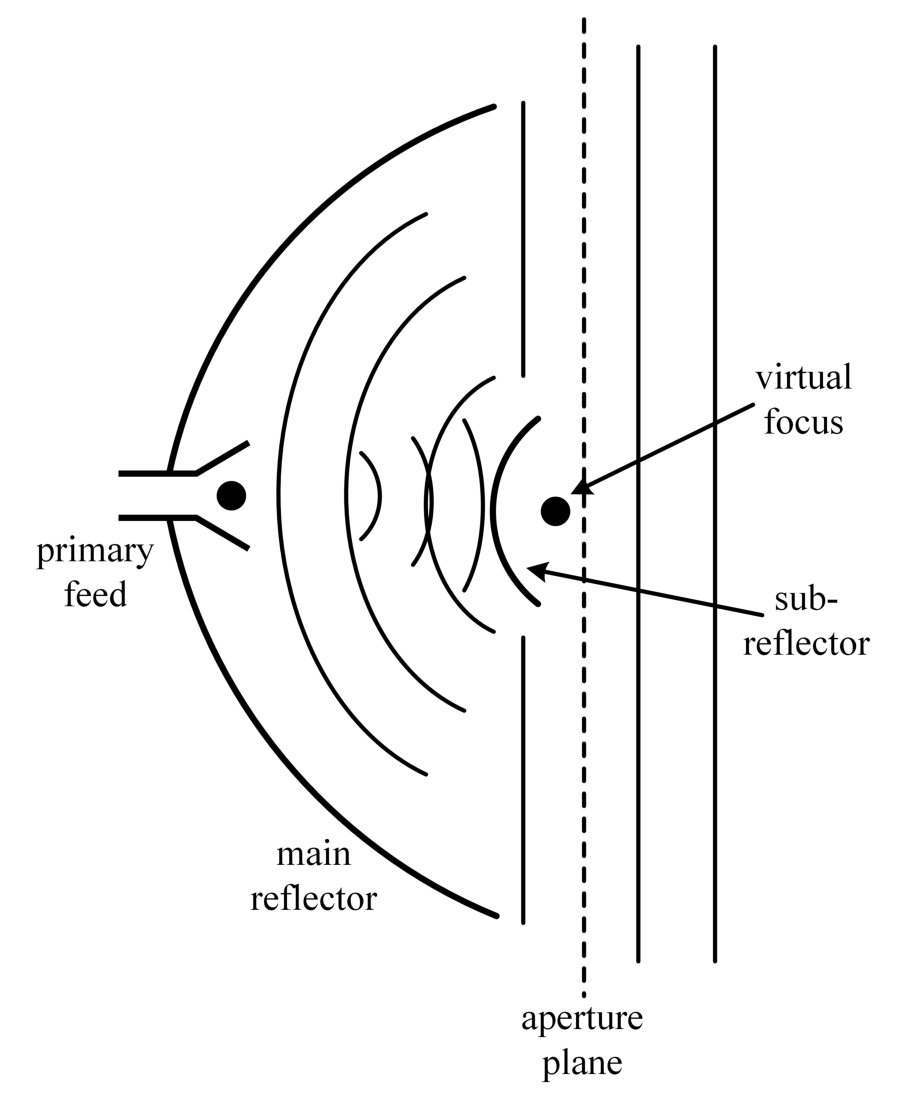
\epsfig{height=3.5in,file=Figs/intro/cassegrain.eps}
	\end{center}
	\caption{The Cassgrain Double Reflector Antenna.}
	\label{fig:cassegrain}
\end{figure}
The primary feed is inserted through the center of the main paraboloidal reflector, thus eliminating long waveguides feeders and their association noise problems. There is also the possibility of simple control of the antenna radiation pattern by appropriately shaping the sub-reflector. But the problem aperture blocking, this time by the sub-reflector and its supports, still remains.\\
\\
\textbf{The Offset-Fed Paraboloid Reflector Antenna}\\
The problem of blocking of the desired aperture field by the feed can be largely overcome by placing the primary feed in an offset position, as indicated in Fig. \ref{fig:offset-feed}, and appropriately restricting the extent of the main reflector. 
\begin{figure}[htbp]
	\begin{center}
		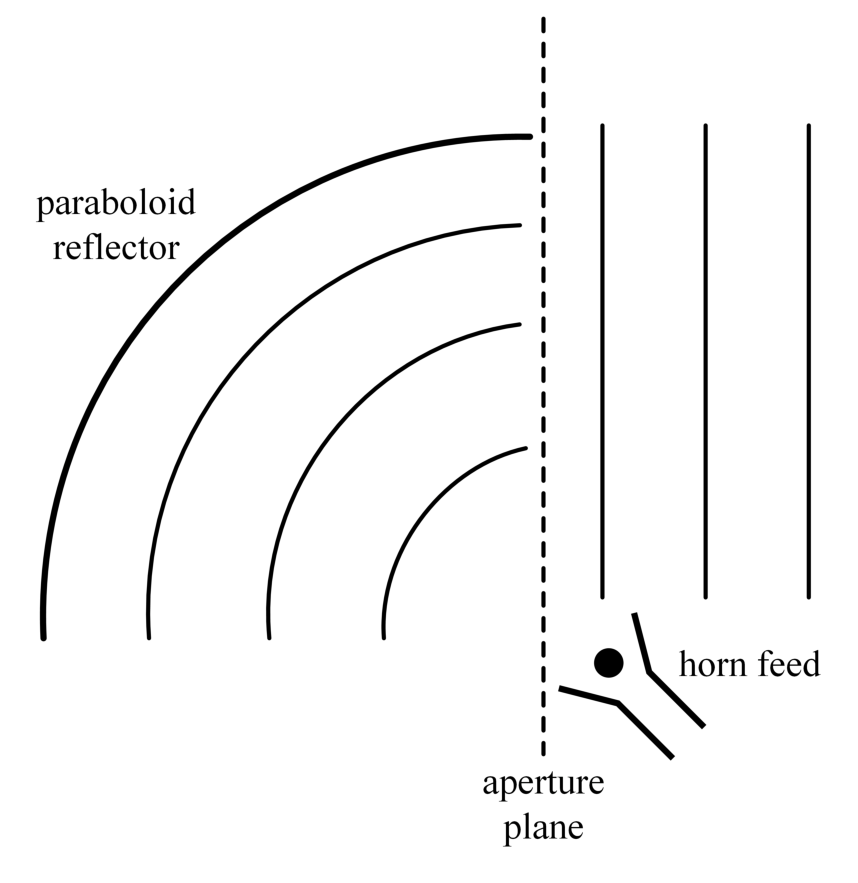
\epsfig{height=3.5in,file=Figs/intro/offset-feed.eps}
	\end{center}
	\caption{The Offset-Fed Paraboloid Reflector Antenna.}
	\label{fig:offset-feed}
\end{figure}
The price to be paid for the resulting improvement is that such an antenna is awkward to manufacture (at least for mass production), and the skew geometry can give rise to increased cross-polarized radiation, which may be undesirable.

Nonetheless, our main concern here is not with the pros and cons of different antennas, but with the common feature that makes them eligible to be considered as aperture antennas; which is that an analysis of their performance arises naturally (but not necessarily exclusively) from consideration of a field distribution over some surface in the vicinity of the antenna structures. This is clearly so in the present instance, as suggested in Fig. \ref{fig:offset-feed}.


\section{Basic Antenna Concepts}
\label{sec:antconc}
The object of antenna analysis is an accuracy description of the radiating and receiving characteristics of an antenna. Over the years certain concepts and definitions have developed and become established as part of the common language among antenna engineers. We will review these concepts and definitions here. They will be developed in detail and discussed at greater length in later chapters.\\
\\
\textbf{The Radiated Far Field}\\
\begin{figure}[htbp]
	\begin{center}
		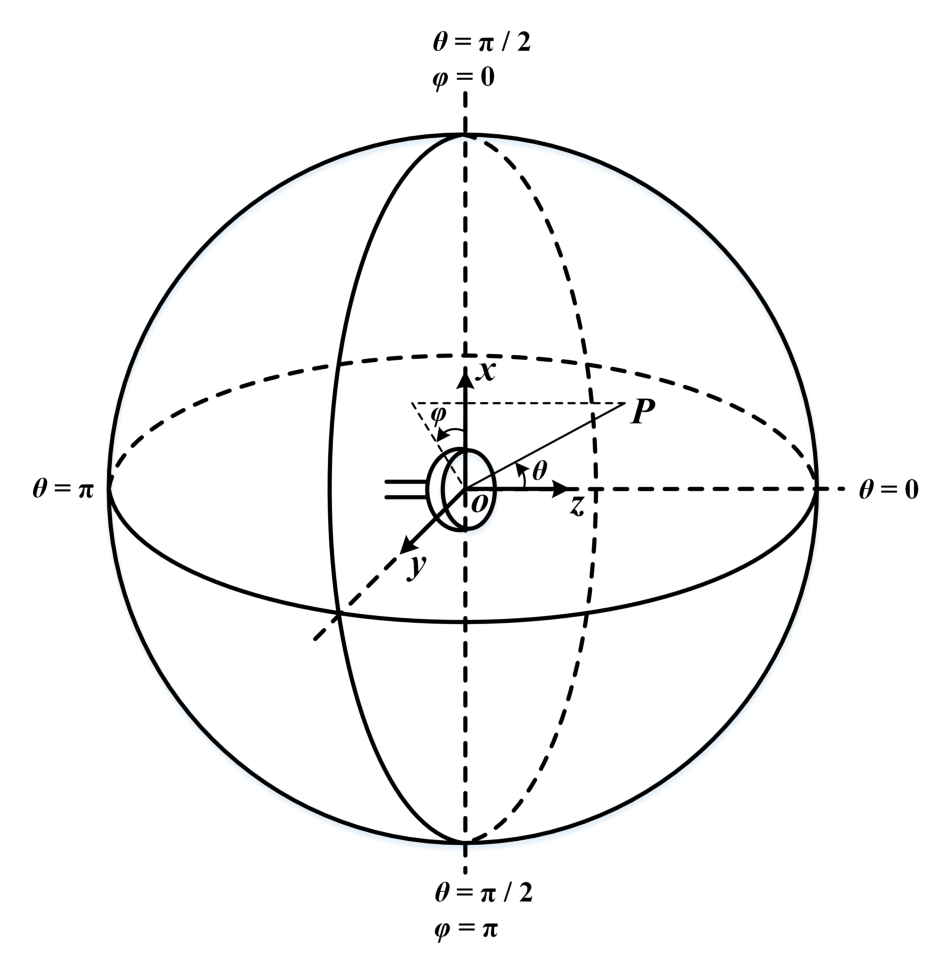
\epsfig{height=4.0in,file=Figs/intro/geo3d.eps}
	\end{center}
	\caption{Geometry for the radiated field.}
	\label{fig:geo3d}
\end{figure}
At a large distance $r$ from any antenna its electric field can be expressed in the form
\begin{subequations}
	\label{eq:radff}
	\begin{equation}
	\mathbf{E}(r,\theta,\phi)=\frac{\exp(-jkr)}{kr}\mathbf{e}(\theta,\phi)
	\label{eq:antffexpr}
	\end{equation}
	such that
	\begin{equation}
	\mathbf{u}_r\cdot\mathbf{E}(r,\theta,\phi)=0,
	\label{eq:tanfd}
	\end{equation}
\end{subequations}
and the associated magnetic field is
\begin{equation}
\mathbf{H}(r,\theta,\phi)=\frac{1}{Z}\mathbf{u}_r\times\mathbf{E}(r,\theta,\phi)
\label{eq:magfd}
\end{equation}
The observation point $P$ (See Fig. \ref{fig:geo3d}) is assumed to lie on a sphere of radius $r$, centered on a convenient point $O$ in the vicinity of the antenna.
The spherical polar coordinates of the point $P$ are $(r,\theta,\phi)$ where $\theta$, the polar angle, and $\phi$, the azimuth angle, together define the direction of $P$ from $O$. The direction $(\theta, \phi)$ is also that of the unit vector in the radial direction, $\mathbf{u}_r$.

The following features of the antenna far field should be noted:
\begin{itemize}
	\item [(a)]
	The distance $r$ of the observation point from the antenna should be at least the Rayleigh distance, which will be shown in section \ref{ssec:tran2ff} to be $2a^2/\lambda$, where $a$ is the maximum dimension of the radiating aperture.
	\item [(b)]
	The time variation of the fields is understood to be sinusoidal, having the complex from $\exp(j\omega t)$. This meas that the actual space-time behavior for a phasor-vector such as $\mathbf{E}(r,\theta,\phi)$ is obtained from
	\begin{equation}
	\mathbf{E}(r,\theta,\phi,t)=\text{Re}[\mathbf{E}(r,\theta,\phi)e^{j\omega t}]
	\end{equation}
	where Re denotes the real part. The convention we are using is that the phasor-vector $\mathbf{E}$ has a complex magnitude $E$ and an absolute magnitude $|E|$, which is also the peak value of the sinusoidal time variation.
	\item [(c)]
	The form of the far electric field $\mathbf{E}(r,\theta,\phi)$ of equation (\ref{eq:antffexpr}) is the product of a uniform spherical scalar wave and the vector pattern function $\mathbf{e}(\theta,\phi)$.
	\item [(d)]
	The dimension of $\mathbf{e}(\theta, \phi)$ are the same as those of $\mathbf{E}(r,\theta,\phi)$, namely volts per meter, as a consequence of arbitrary multiplying $r$ in the denominator of equation equation (\ref{eq:antffexpr}) by the plane-wave phase constant $k=\omega \sqrt{\mu \epsilon}$.
	\item [(e)]
	In a particular direction $(\theta,\phi)$ the amplitude of the field falls off as $r^{-1}$, and its phase is retarded linearly as $kr$, with increasing radial distance $r$.
	\item [(f)]
	At a constant radial distance the dependence on direction of the amplitude, phase and polarization (that is, vector direction) of the electric field is given by $\mathbf{e}(\theta,\phi)$, which is the vector pattern function for a particular antenna.
	\item [(g)]
	The electric field $\mathbf{E}(r,\theta,\phi)$ is polarized such that it is always tangential to the sphere of radius $r$, as specified by equation (\ref{eq:tanfd}). This is illustrated in Fig. \ref{fig:pol-rh}.
	\begin{figure}[htbp]
		\begin{center}
			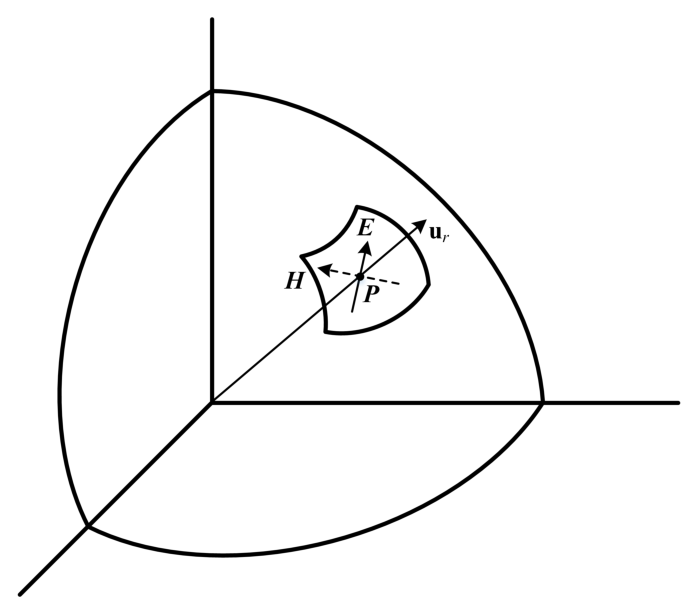
\epsfig{height=3.0in,file=Figs/intro/pol-rh.eps}
		\end{center}
		\caption{Polarization of the far field. $\mathbf{E}$, $\mathbf{H}$, and $\mathbf{u}_r$ form a right-handed set.} 
		\label{fig:pol-rh}
	\end{figure}
	\item [(h)]
	The magnetic field $\mathbf{H}(r,\theta,\phi)$ of equation (\ref{eq:magfd}) is also tangential to the sphere of radius $r$. It is also orthogonal to $\mathbf{E}(r,\theta,\phi)$. The $\mathbf{E}$, $\mathbf{H}$ and $\mathbf{u}_r$ are mutually orthogonal everywhere in the far field. They form a right-handed set in the stated order (that is, if $\mathbf{E}$ is rotated on to $\mathbf{H}$, a right-handed screw thread would advantage in the direction of $\mathbf{u}_r$) as specified by equation (\ref{eq:radff}) and (\ref{eq:magfd}) and illustrated in Fig. \ref{fig:pol-rh}.
	\item [(i)]
	In equation (\ref{eq:magfd}), which relates the electric and magnetic fields, $Z$ is the plane-wave impedance of the propagating medium. In terms of the permeability $\mu$ and permittivity $\epsilon$ of the medium,
	\begin{equation}
	Z = \sqrt{\dfrac{\mu}{\epsilon}}
	\end{equation}
	\item [(j)]
	In the neighborhood of any point $\mathbf{P}$ in the field the electric and magnetic fields have the {\itshape local} character of a plane wave traveling in the radial direction.
	\item [(k)]
	The power flux density, given by half the real part of the complex Poynting vector
	\begin{equation}
	\mathbf{S}=\frac{1}{2}\text{ Re }\mathbf{E}\times\mathbf{H^*},
	\end{equation}
	is directed radially outward (this is, $\mathbf{S}=\mathbf{u}_rS_r$) for the values of $\mathbf{E}$ and $\mathbf{H}$ given above for the far field. The asterisk denotes complex conjugate. The radial component of the power flux density is therefore
	\begin{equation}
	S_r(r,\theta,\phi)=\dfrac{\mathbf{e}(\theta,\phi)\cdot\mathbf{e}^*(\theta,\phi)}{2(kr)^2Z}=\dfrac{|e(\theta,\phi)^2|}{2(kr)^2Z}
	\end{equation}
\end{itemize}
\textbf{Directivity, Gain and Efficiency}\\
The directivity $D(\theta,\phi)$ of a radiating antenna is defined as the ratio:\\
\begin{equation}
D(\theta,\phi)=\frac{\mathrm{Power\ flux\ density\ (p.f.d)\ from\ antenna\ in\ direction\ (\theta,\phi)}}{\mathrm{P.f.d.\ when\ same\ power\ is\ radiated\ uniformly\ in\ all\ directions}}.
\label{eq:dir}
\end{equation}
The power flux densities in this definition must be measured at the same radial distance, or equivalently the power flux density must be defined per unit solid angle. In either case the definition refers to the far field.

If $P_t$ is the total power radiated by the antenna, the power flux density at a distance $r$ when this is radiated uniformly in all directions (that is, radiated isotropically) is
\begin{equation}
S_r^{iso}(r,\theta,\phi)=\frac{P_t}{4\pi r^2},
\end{equation}
and the antenna directivity is
\begin{equation}
D(\theta,\phi)=\dfrac{S_r(r,\theta,\phi)}{S_r^{iso}(r,\theta,\phi)}=\dfrac{\lambda^2|e(\theta,\phi)|^2}{2\pi ZP_t}
\label{eq:dirdetial}
\end{equation}
for the far fields defined earlier.

Antenna gain $G(\theta,\phi)$ has a definition similar to that of directivity, the only difference being that the denominator of equation (\ref{eq:dir}) is based on the input power $P_{in}$ delivered to the antenna. Thus
\begin{equation}
G(\theta,\phi)=\eta D(\theta,\phi) ; 0\leqslant \theta \leqslant 1,
\end{equation}
where $\eta$, know as the antenna efficiency, is the ratio of total power radiated to the power input to the antenna, namely,
\begin{equation}
\eta = P_t/P_{in}
\end{equation}
In terms of the far-field pattern function, then,
\begin{equation}
G(\theta,\phi)=\dfrac{\lambda^2|e(\theta,\phi)|^2}{2\pi ZP_{in}}
\label{eq:gain}
\end{equation}
The maximum value of the gain function $G(\theta,\phi)$ is also often referred to simply as the gain of the antenna.

The polarization of the far field is described by the complex vector $\mathbf{e}(\theta,\phi)$, which is constrained to lie in a plane perpendicular to the radial direction. The vector, $\mathbf{e}$ can therefore be resolved into two components with basis vector $\mathbf{e}_1$ and $\mathbf{e}_2$, so that
\begin{equation}
\mathbf{e}=a_1\mathbf{e}_1+a_2\mathbf{e}_2
\end{equation}
in which $a_1$ and $a_2$ are complex. The basis vectors can be so chosen that they are normalized with
\begin{equation}
\mathbf{e}_1\cdot{\mathbf{e}_1}^*=\mathbf{e}_2\cdot{\mathbf{e}_2}^*=1
\end{equation}
and orthogonal in the sense that
\begin{equation}
\mathbf{e}_1\cdot{\mathbf{e}_2}^*=\mathbf{e}_2\cdot{\mathbf{e}_1}^*=0 .
\end{equation}
This resolution of the field could be into two orthogonal linearly polarized plane waves, or into a combination of right-hand and left-hand circularly polarized plane waves, whichever is more appropriate. Then
\begin{equation}
\mathbf{e}\cdot{\mathbf{e}}^*=|a_1|^2+|a_2|^2=|e|^2
\end{equation}
and it is clear from equation (\ref{eq:dirdetial}) that the directivity can be resolved into two parts, namely,
\begin{equation}
D(\theta,\phi)=D_1(\theta,\phi)+D_2(\theta,\phi)
\end{equation}
based on the chosen resolution of the field. Equation (\ref{eq:gain}) shows that the gain $G(\theta,\phi)$ can be similarly resolved.\\
\\
\textbf{Radiation Patterns, Beamwidth and Sidelobes}\\
It is usually required of an antenna that it be directive. The simplest measure of its effectiveness as such is the gain, that is, the maximum value of the gain function $G(\theta,\phi)$. The gain is thus the ratio, invariably stated in decibels (dB), of the maximum power flux density produced by the antenna to its value if the power delivered to the antenna had been radiated isotropically.

More information about its directive properties can be obtained from the antenna's radiation patterns. There are plots of radiated field strength or, more usually, power flux density (directivity or gain) as a function of angle. Since direction is specified by two angles whereas it is only possible to plot against one, antenna radiation patterns consist of a set of section in the $\theta\textendash\phi$, or some equivalent, plane. For example, suppose that an antenna has its maximum power radiation in the direction $\theta=0$. Then a plot of the antenna gain, in decibels relative to the maximum value, as a function of $\theta$ with $\phi$ held constant might be that sketched in Fig. \ref{fig:pol-rec}.
\begin{figure}[htbp]
	\begin{center}
		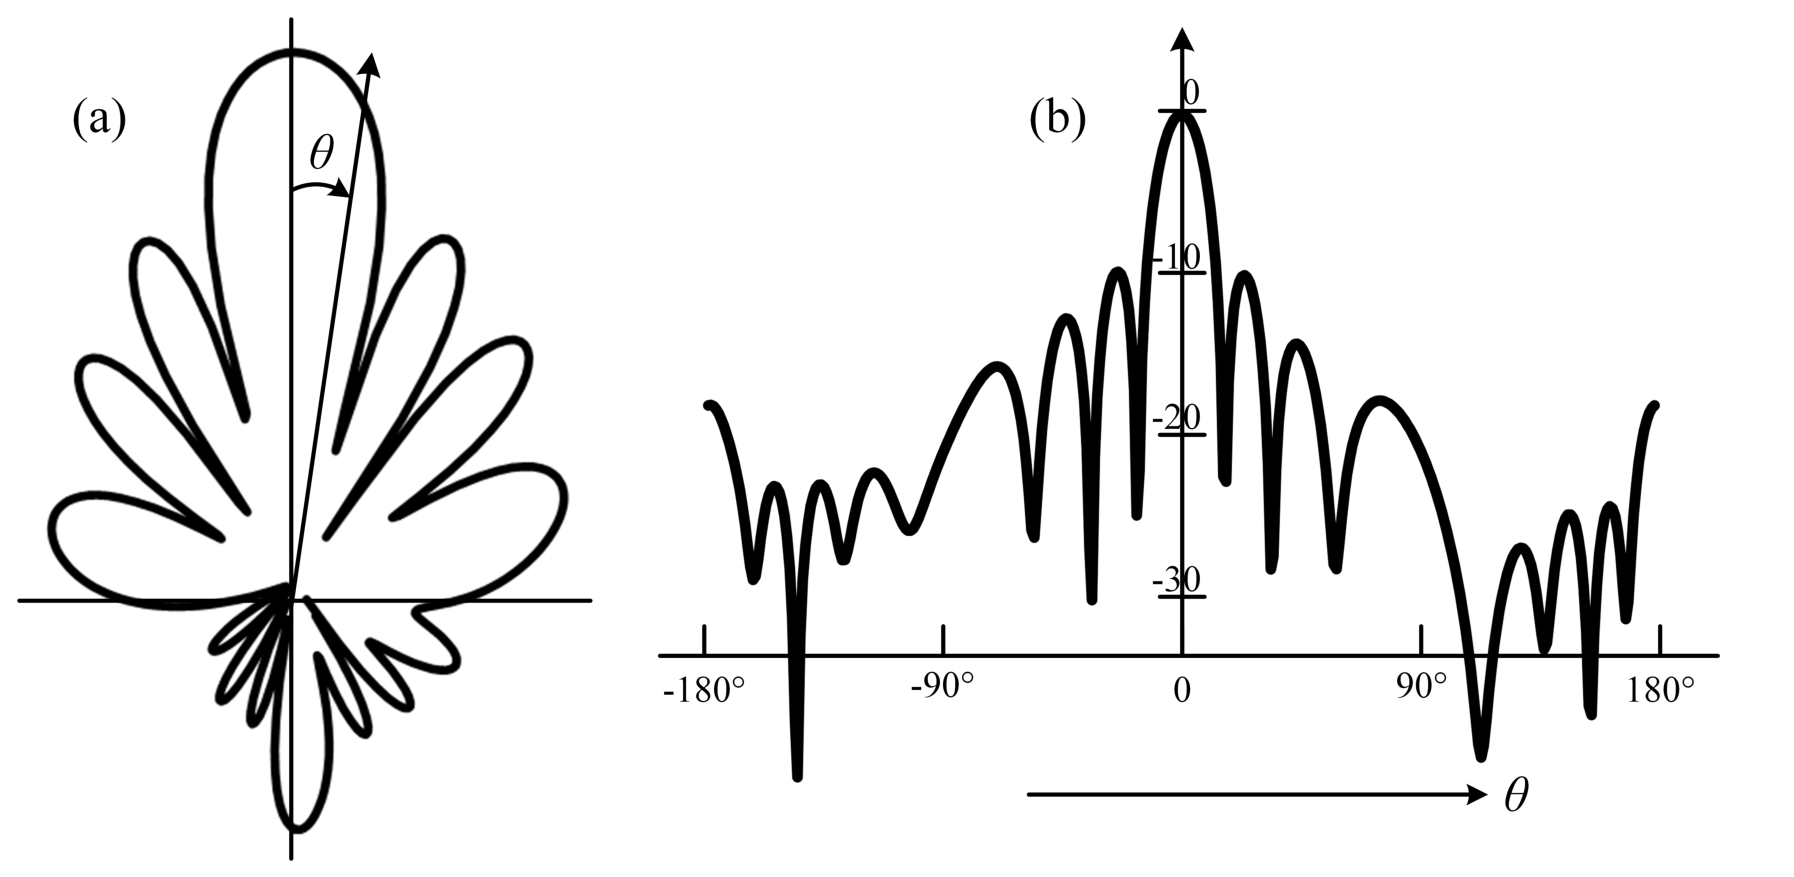
\epsfig{width=4.0in,file=Figs/intro/pol-rec.eps}
	\end{center}
	\caption{Polar and rectangular plts of relative gain in dB versus for constant $\phi$.} 
	\label{fig:pol-rec}
\end{figure}
Two methods of plotting the same information are shown, one in polar the other in rectangular form.

Antenna radiation patterns often have a lobe structure similar to that shown. The lobe containing the direction of maximum radiated power is the main lobe; all other lobes are referred to as sidelobes. The two sidelobes adjacent to the main lobe are the first sidelobes, and the lobe diametrically opposite the main lobe, if it exists, is called the back lobe. The lobes are separated by nulls, so called because the power radiated in these directions can in theory be zero.
\begin{figure}[htbp]
	\begin{center}
		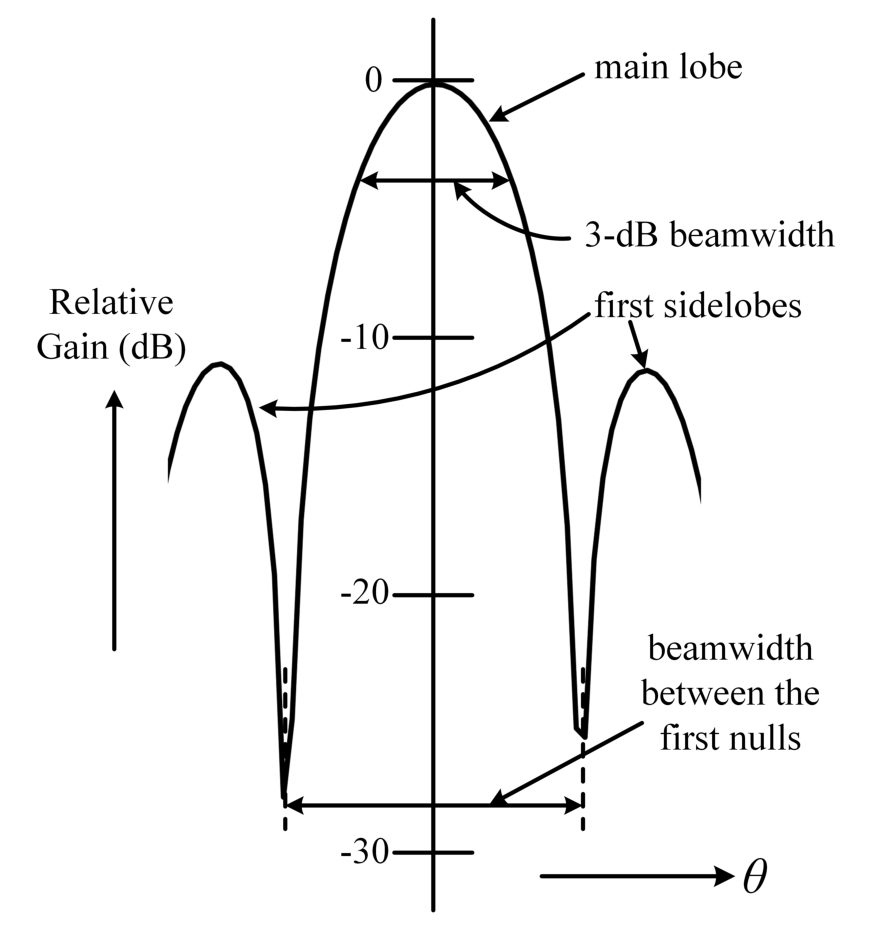
\epsfig{height=3.0in,file=Figs/intro/lobes.eps}
	\end{center}
	\caption{Details of the main lobe and first sidelobes of the antenna pattern in Fig. \ref{fig:pol-rec}(b). showing two ways of defining antenna beamwidth.} 
	\label{fig:lobes}
\end{figure}
The angular width of the main lobe of the antenna, known as its beam width, is a useful measure of the capability of the antenna of resolving the angular position of a distant point source. Two common ways of defining antenna beamwidth are shown in Fig. \ref{fig:lobes}. One is the angle between the two points on either side of the main lobe at which the radiated power has fallen to half its maximum value, that is, the -3 dB points, and is known as the 3-dB beamwidth. The other definition is the angle between the first nulls of the pattern, which is usually about twice the 3-dB beamwidth. This fact makes the additional point that if two distant sources are separated in angle by the 3-dB beamwidth and one of them lies in the center of the main beam, then the other will lie in the region of the first null.\\
\\
\textbf{Receiving Antennas}\\
The directivity of a receiving antenna is defined in terms of its response to an incident plane wave. It takes the form of an effective receiving area:
\begin{equation}
A(\theta,\phi)=\frac{\mathrm{Power\ delivered\ to\ receiver}}{\mathrm{Power\ density\ in\ plane\ wave\ incident\ from\ direction\ (\theta,\phi)}}
\end{equation}
It is assumed that the polarization of the incident plane wave is adjusted to deliver maximum power to the receiver: a condition known as \textbf{polarization match}.

Consider the plane wave to be $\mathbf{E}'$, incident from the direction $(\theta', \phi')$, as shown in Fig. \ref{fig:receive}. 
\begin{figure}[htbp]
	\begin{center}
		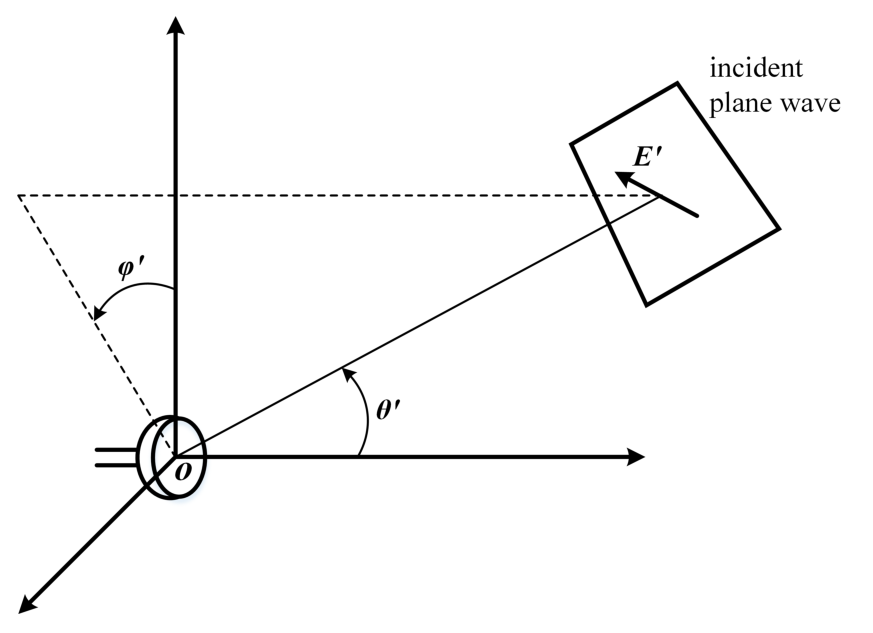
\epsfig{width=3.5in,file=Figs/intro/receive.eps}
	\end{center}
	\caption{Plane wave incident on a receiving antenna.} 
	\label{fig:receive}
\end{figure}
If the antenna has a vector far-field radiation pattern $\mathbf{e}(\theta,\phi)$, the antenna reciprocity theorem of section \ref{ssec:recitheo} states that the received signal will be proportional to $\mathbf{E}'\cdot\mathbf{e}(\theta',\phi')$. The vector $\mathbf{E}'$ and $\mathbf{e}(\theta',\phi')$ lies in the same plane; the condition of polarization match is therefore when they are coincident in that plane. When this occurs the power delivered to the receiver will be proportional to $|E'|^2\cdot|e(\theta',\phi')|$, which means that it is proportional to the product of the power density in the incident plane wave and the gain of the antenna given by equation (\ref{eq:gain}). Thus the effective receiving area of an antenna proportional to its transmitting gain. The precise relationship will be shown in section \ref{ssec:gainfunc} to be
\begin{equation}
A(\theta,\phi)=\dfrac{\lambda^2}{4\pi}G(\theta,\phi)
\label{eq:Atp}
\end{equation}
\\
\textbf{Transmitter to Receiver Coupling}\\
An immediate use for the definition we have just given of antenna gain and receiving area is the far-field coupling equation, known as the \textbf{Friis transmission formula} which we will now derive. (This is a particular form of a more general result that will be obtained later in section \ref{sec:coupling}).

Suppose that the transmitting and receiving antennas are disposed as shown in Fig. \ref{fig:coupling}.
\begin{figure}[htbp]
	\begin{center}
		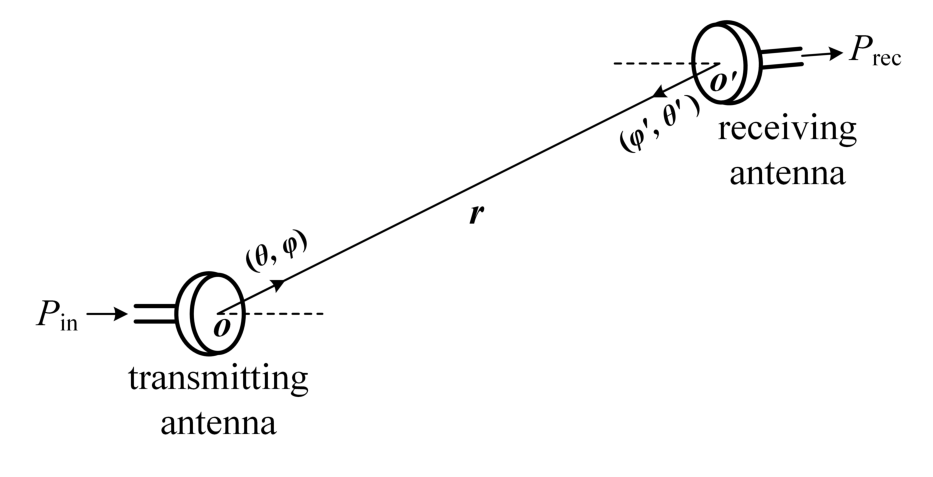
\epsfig{width=3.5in,file=Figs/intro/coupling.eps}
	\end{center}
	\caption{Plane wave incident on a receiving antenna.} 
	\label{fig:coupling}
\end{figure}
The distance $r$ between them is presumed to satisfy the far-field criterion that $r\geqslant2a^2/\lambda$, where $a$ is now the largest dimension of both antenna apertures. The receiver is in the direction $\theta,\phi$ from the transmitter, and the transmitter is in the direction $(\theta',\phi')$ from the receiver; and if the transmitting antenna gain is $G_T(\theta,\phi)$, when $P_{in}$ is delivered to the transmitter, the power flux density incident on the receiving antenna in the form of a locally plane wave will be
\begin{equation}
S_r=P_{in}\dfrac{G_T(\theta,\phi)}{4\pi r^2}
\end{equation}
If the effective receiving area of the receiving antenna is $A_R(\theta',\phi')$, the power delivered to the receiver will be
\begin{equation}
P_{rec}=P_{in}\dfrac{G_T(\theta,\phi)A_R(\theta',\phi')}{4\pi r^2},
\end{equation}
it being assumed that the receiving antenna is polarization matched to the incident field. An alternative form for the received power, using equation (\ref{eq:Atp}) is 
\begin{equation}
P_{rec}=P_{in}\dfrac{\lambda^2G_T(\theta,\phi)G_R(\theta',\phi')}{{4\pi}^2r^2}
\end{equation}

\begin{figure}[htbp]
	\begin{center}
		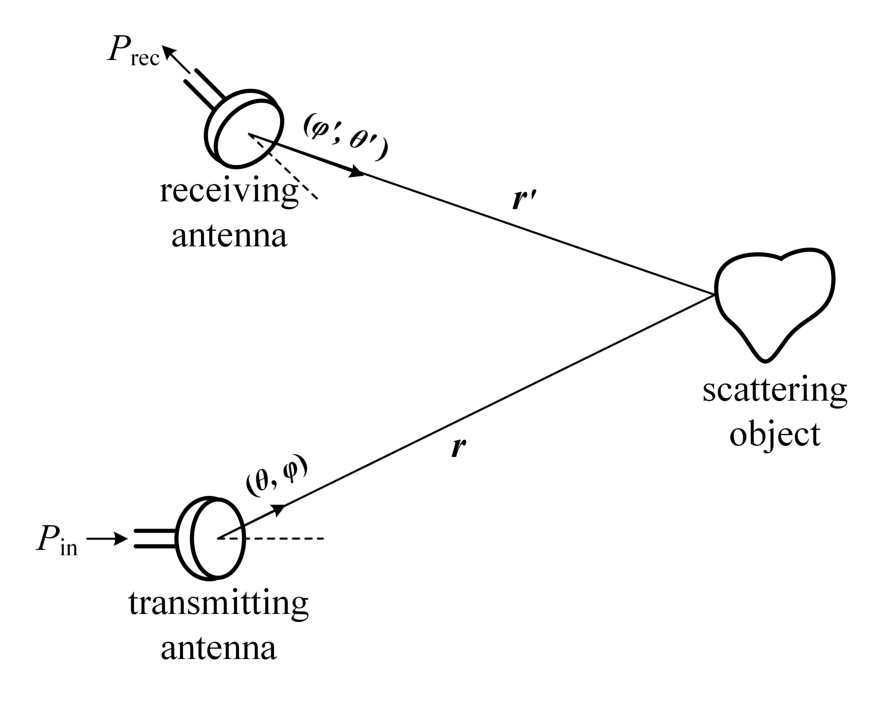
\epsfig{height=3.0in,file=Figs/intro/scattering.eps}
	\end{center}
	\caption{Geometry for the indirect coupling between a transmitting and receiving antenna via a scattering object.} 
	\label{fig:scattering}
\end{figure}
Another important form of coupling between a transmitter and a receiver occurs indirectly via a scattering object, as in radar. The scatterer is represented by its \textbf{scattering cross-section}, which has the following rather tortuous but basically simple definition. The scattering cross-section $\sigma$ is that area which, when placed perpendicular to the plane-wave field incident on the scatterer, would intercept that amount of power which, when radiated uniformly in all directions, would give the observed power flux density in a particular direction, it is therefore a function of the direction and polarization of the incident field, and of the direction of observation.

If, with the geometry show in Fig. \ref{fig:scattering}, power $P_{in}$ is delivered to the transmitting antenna and the scatterer is in its far field, the power intercepted will be $P_{in}G_T(\theta,\phi)\sigma/4\pi r^2$, and the power delivered to the receiver will be therefore be
\begin{equation}
P_{rec}=P_{in}\dfrac{\sigma G_T(\theta,\phi)G_R(\theta',\phi')}{{4\pi}^2r^2{r'}^2},
\end{equation}
again assuming that the receiving antenna is polarization matched to the field incident upon it. In radar systems the same antenna is often used for transmitting and receiving, in which case the received power is
\begin{equation}
P_{rec}=P_{in}\dfrac{\lambda^2G^2(\theta,\phi)}{{4\pi}^3r^4},
\end{equation}
where we have set $G_T(\theta,\phi)=G_R(\theta,\phi)=G(\theta,\phi), r'=r$ and have made use of equation (\ref{eq:Atp}).